\section{More About Lattices}

\begin{parts}
\item We don't even really need to draw anything for the first case. In the ferromagnetic case, all lattice sites are equivalent, so the unit cell is simply a single unit square of length $a$, meaning

  
  \begin{equation}
    A_0 = a^2,\ \text{and}\ A_{\mathrm{BZ}} = \frac{(2\pi)^2}{A_0} = \left( \frac{2\pi}{a} \right)^2.
  \end{equation}

  \begin{figure}
    \centering
    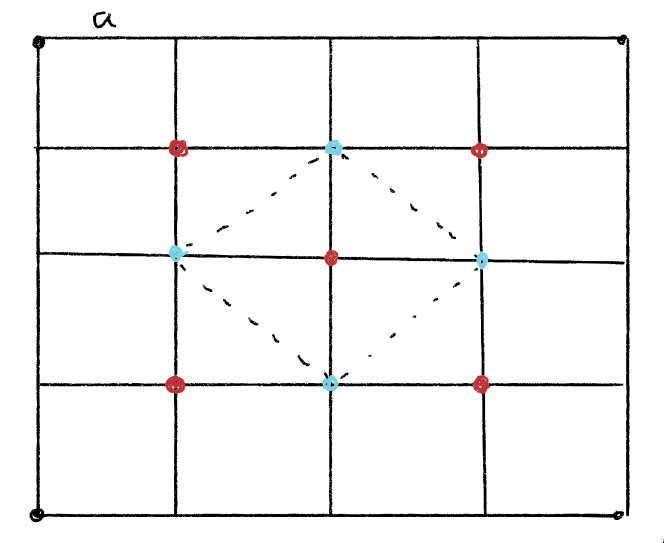
\includegraphics[width=0.6\linewidth]{./res/Pics/5-a.png}
    \caption{}\label{fig:5-a}
  \end{figure}

  In the anti-ferromagnatic case, the lattice sites are not equivalent -- they look like Fig.~\ref{fig:5-a}. In this case, then, are unit cell looks a bit different. In particular, it is another square connecting identical lattice sites, but the side length is $a\sqrt{2}$ this time. Therefore,

  \begin{equation}
    A_0 = 2a^2,\ \text{and}\ A_{\mathrm{BZ}} = \frac{(2\pi)^2}{A_0} = \frac{1}{2}\left( \frac{2\pi}{a} \right).
  \end{equation}

  As we would expect, the area of the primitive cells in this case are larger, so the corresponding area in the reciprocal space is smaller.



\item This part is drawn in Fig.~\ref{fig:5-b}.

  \begin{figure}
    \centering
    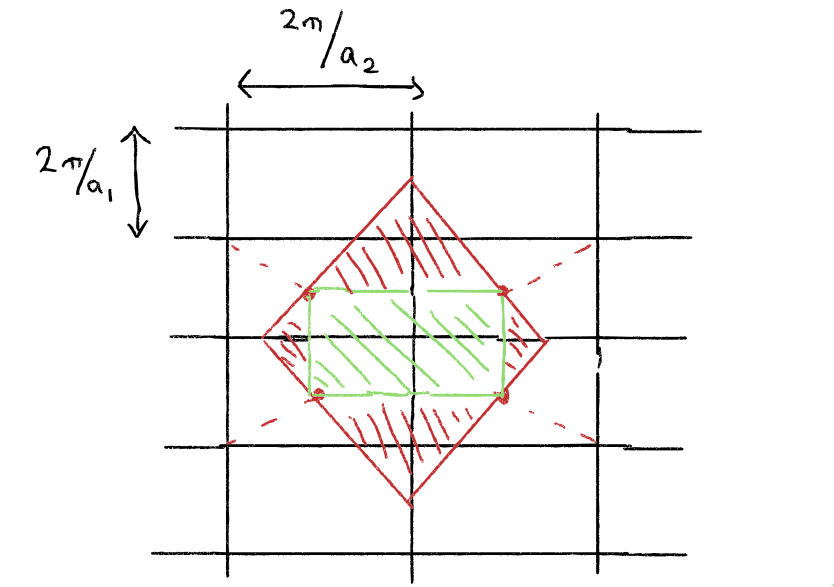
\includegraphics[width=0.6\linewidth]{./res/Pics/5-b.png}
    \caption{}\label{fig:5-b}
  \end{figure}




\item The atomic packing factor is defined as

  \begin{equation}
    \mathrm{APF} = \frac{N_{ac}V_a}{V_c},
  \end{equation}

  where $N_{a/c}$ is the number of atoms in a unit cell, $V_a$ is the volume of the atom, and $V_c$ is the volume of the unit cell. We first note that we can approximate our atoms as spheres of radius $r$, so $V_c = 4\pi r^3/3$ for each lattice. Also, I am using the visuals from the lecture notes to assist with my determination of some lengths.

  First, for the SC lattice, in our unit cell, we grab $1/8$th of each atom at each corner, of which there are 8, meaning we have 1 atom per unit cell. The length of the unit cell is two halfs of each atom, so it is simply $2r$. Thus:

  \begin{equation}
    \mathrm{APF}_{\mathrm{SC}} = \frac{1 \cdot 4\pi r^3/3}{(2r)^3} = \frac{4}{3\cdot8}\pi = \frac{\pi}{6}.
  \end{equation}

  For the BCC, we have an additional atom in the center of the unit cell, so there are 2 atoms per unit cell. The length of the diagonal from the center of the unit cell to the center of the call a corner is $2r$, so the total diagonal is $4r$, meaning the length of the side is $4r/\sqrt{3}$. With this:

  \begin{equation}
    \mathrm{APF}_{\mathrm{BCC}} = \frac{2 \cdot 4\pi r^3/3}{(4r/\sqrt{3})^3} = \frac{8}{3} \cdot \frac{3\sqrt{3}}{64}\pi = \frac{\pi\sqrt{3}}{8}.
  \end{equation}

  Lastly, for the FCC, instead of an atom at the center, we have half of an atom on each face, so an additional 3 atoms compared to the SC for a total of 4 atoms in the unit cell. From this, we have that the diagonal of one of the sides is $4r$, meaning a side length is $4r/\sqrt{2} = 2r\sqrt{2}$, so

  \begin{equation}
    \mathrm{APF}_{\mathrm{FCC}} = \frac{4 \cdot 4\pi r^3/3}{(2r\sqrt{2})^3} = \frac{16}{3} \frac{1}{16\sqrt{2}}\pi = \frac{\pi\sqrt{2}}{6}.
  \end{equation}
\end{parts}

%%% Local Variables:
%%% mode: LaTeX
%%% TeX-master: "../../HW3"
%%% End:
